
\documentclass[a4paper,11pt]{article}
\usepackage[a4paper, margin=8em]{geometry}

% usa i pacchetti per la scrittura in italiano
\usepackage[french,italian]{babel}
\usepackage[T1]{fontenc}
\usepackage[utf8]{inputenc}
\frenchspacing 

% usa i pacchetti per la formattazione matematica
\usepackage{amsmath, amssymb, amsthm, amsfonts}

% usa altri pacchetti
\usepackage{gensymb}
\usepackage{hyperref}
\usepackage{standalone}

% imposta il titolo
\title{Appunti Fondamenti di Automatica}
\author{Luca Seggiani}
\date{2025}

% disegni
\usepackage{pgfplots}
\pgfplotsset{width=10cm,compat=1.9}

% imposta lo stile
% usa helvetica
\usepackage[scaled]{helvet}
% usa palatino
\usepackage{palatino}
% usa un font monospazio guardabile
\usepackage{lmodern}

% tikz in sans
\tikzset{every picture/.style={/utils/exec={\sffamily}}}

\renewcommand{\rmdefault}{ppl}
\renewcommand{\sfdefault}{phv}
\renewcommand{\ttdefault}{lmtt}

% circuiti
\usepackage{circuitikz}
\usetikzlibrary{babel}

% disponi il titolo
\makeatletter
\renewcommand{\maketitle} {
	\begin{center} 
		\begin{minipage}[t]{.8\textwidth}
			\textsf{\huge\bfseries \@title} 
		\end{minipage}%
		\begin{minipage}[t]{.2\textwidth}
			\raggedleft \vspace{-1.65em}
			\textsf{\small \@author} \vfill
			\textsf{\small \@date}
		\end{minipage}
		\par
	\end{center}

	\thispagestyle{empty}
	\pagestyle{fancy}
}
\makeatother

% disponi teoremi
\usepackage{tcolorbox}
\newtcolorbox[auto counter, number within=section]{theorem}[2][]{%
	colback=blue!10, 
	colframe=blue!40!black, 
	sharp corners=northwest,
	fonttitle=\sffamily\bfseries, 
	title=Teorema~\thetcbcounter: #2, 
	#1
}

% disponi definizioni
\newtcolorbox[auto counter, number within=section]{definition}[2][]{%
	colback=red!10,
	colframe=red!40!black,
	sharp corners=northwest,
	fonttitle=\sffamily\bfseries,
	title=Definizione~\thetcbcounter: #2,
	#1
}

% disponi problemi
\newtcolorbox[auto counter, number within=section]{problem}[2][]{%
	colback=green!10,
	colframe=green!40!black,
	sharp corners=northwest,
	fonttitle=\sffamily\bfseries,
	title=Problema~\thetcbcounter: #2,
	#1
}

% disponi codice
\usepackage{listings}
\usepackage[table]{xcolor}

\lstdefinestyle{codestyle}{
		backgroundcolor=\color{black!5}, 
		commentstyle=\color{codegreen},
		keywordstyle=\bfseries\color{magenta},
		numberstyle=\sffamily\tiny\color{black!60},
		stringstyle=\color{green!50!black},
		basicstyle=\ttfamily\footnotesize,
		breakatwhitespace=false,         
		breaklines=true,                 
		captionpos=b,                    
		keepspaces=true,                 
		numbers=left,                    
		numbersep=5pt,                  
		showspaces=false,                
		showstringspaces=false,
		showtabs=false,                  
		tabsize=2
}

\lstdefinestyle{shellstyle}{
		backgroundcolor=\color{black!5}, 
		basicstyle=\ttfamily\footnotesize\color{black}, 
		commentstyle=\color{black}, 
		keywordstyle=\color{black},
		numberstyle=\color{black!5},
		stringstyle=\color{black}, 
		showspaces=false,
		showstringspaces=false, 
		showtabs=false, 
		tabsize=2, 
		numbers=none, 
		breaklines=true
}

\lstdefinelanguage{javascript}{
	keywords={typeof, new, true, false, catch, function, return, null, catch, switch, var, if, in, while, do, else, case, break},
	keywordstyle=\color{blue}\bfseries,
	ndkeywords={class, export, boolean, throw, implements, import, this},
	ndkeywordstyle=\color{darkgray}\bfseries,
	identifierstyle=\color{black},
	sensitive=false,
	comment=[l]{//},
	morecomment=[s]{/*}{*/},
	commentstyle=\color{purple}\ttfamily,
	stringstyle=\color{red}\ttfamily,
	morestring=[b]',
	morestring=[b]"
}

% disponi sezioni
\usepackage{titlesec}

\titleformat{\section}
	{\sffamily\Large\bfseries} 
	{\thesection}{1em}{} 
\titleformat{\subsection}
	{\sffamily\large\bfseries}   
	{\thesubsection}{1em}{} 
\titleformat{\subsubsection}
	{\sffamily\normalsize\bfseries} 
	{\thesubsubsection}{1em}{}

% disponi alberi
\usepackage{forest}

\forestset{
	rectstyle/.style={
		for tree={rectangle,draw,font=\large\sffamily}
	},
	roundstyle/.style={
		for tree={circle,draw,font=\large}
	}
}

% disponi algoritmi
\usepackage{algorithm}
\usepackage{algorithmic}
\makeatletter
\renewcommand{\ALG@name}{Algoritmo}
\makeatother

% disponi numeri di pagina
\usepackage{fancyhdr}
\fancyhf{} 
\fancyfoot[L]{\sffamily{\thepage}}

\makeatletter
\fancyhead[L]{\raisebox{1ex}[0pt][0pt]{\sffamily{\@title \ \@date}}} 
\fancyhead[R]{\raisebox{1ex}[0pt][0pt]{\sffamily{\@author}}}
\makeatother

\begin{document}

% sezione (data)
\section{Lezione del 08-04-25}

% stili pagina
\thispagestyle{empty}
\pagestyle{fancy}

% testo
Ritorniamo sul criterio di Routh.

\subsubsection{Criterio di Routh simbolico}
Il criterio di Routh torna particolarmente utile quando il polinomio studiato ha un coefficiente simbolico.
Ad esempio prendiamo la funzione di trasferimento in ciclo aperto:
$$
G_{OL} = \frac{K_c}{(s + 1)(\frac{s}{2} + 1)(\frac{s}{3} + 1)}
$$
I poli del ciclo aperto sono banali in quanto il polinomio al denominatore è gia fattorizzato ($p_{1,2,3} = 1,2,3$).
Calcoliamo allora i poli al denominatore della retroazione:
$$
1 + G_{OL} = 1 + \frac{K_c}{(s + 1)(\frac{s}{2} + 1)(\frac{s}{3} + 1)} = 
\frac{ s^3 + 6 s^2 + 11s + 6 ( 1 + K_c ) }{ (s + 1)(\frac{s}{2} + 1)(\frac{s}{3} + 1) } 
$$
Come notiamo, compare il parametro $K_c$ al termine noto.
Applichiamo allora il criterio di Routh:
$$
\begin{array}{c | c c}
		3 & 1 & 11 \\
		2 & 6 & 6(1 + K_c) \\
		1 & 10 - K_c \\
		0 & 6(1 + K_c)
\end{array}
$$
Vorremo quindi impostare il sistema:
\[
	\begin{cases}
		10 - K_c > 0 \\
		6(1 + K_c) > 0
	\end{cases}
\]
da cui $-1 < K_c < 10$ è il range in cui il polinomio non ha radici positive.

\par\medskip

\noindent
\begin{minipage}{\textwidth}
Vediamo che quello che abbiamo fatto è effettivamente prendere il sistema:

\begin{center}
	\begin{tikzpicture}
		\draw (1,0) rectangle (3, 1);
		\node at (2, 0.5) {$G(s)$};
		
		\draw (-3,0) rectangle (-1, 1);
		\node at (-2, 0.5) {$K_c$};

		\draw (-1.5, -0.5) rectangle (0.5, -1.5);
		\node at (-0.5, -1) {$H(s) = 1$};

		\draw[-stealth] (-7, 0.5) -> (-5.1, 0.5);
		\draw[-stealth] (-5, 0.5) -> (-3, 0.5);
		\draw[-stealth] (-1, 0.5) -> (1, 0.5);
		\draw[-stealth] (3, 0.5) -> (7, 0.5);
		
		\draw (5, 0.5) -> (5, -1);
		\draw[-stealth] (5, -1) -> (0.5, -1);
		\draw (-1.5, -1) -> (-5, -1);
		\draw[-stealth] (-5, -1) -> (-5, 0.5);

		\draw[fill=white] (-5, 0.5) circle (0.1);


		\node at (-4.75, 0.75) {$+$};
		\node at (-4.75, 0.25) {$-$};

	\end{tikzpicture}
\end{center}
\end{minipage}

\par\medskip
\noindent
a sensore unitario, con la $G(s)$:
$$
G(s) = \frac{G_{OL}}{K_c} = \frac{1}{(s + 1)(\frac{s}{2} + 1)(\frac{s}{3} + 1)}
$$
e tarare il componente $K_c$, che chiamiamo \textit{proporzionale}, in modo da arrivare alla stabilità del sistema.

\subsubsection{Casi singolari del criterio di Routh}
Vediamo alcuni casi particolari del criterio di Routh.
\begin{itemize}
\item \textbf{Primo termine di una riga nullo:} in questo caso il problema sarà che è nullo il pivot per la costruzione della nuova tabella, e ci troveremmo a dividere per zero.
In questo caso possiamo sostituire gli 0 con $\epsilon$ piccoli a piacere.
Portiamo quindi avanti i calcoli conservando zero, e calcolando i termini successivi prendendo il limite $\epsilon \rightarrow 0^+$.
Ad esempio:
$$
\begin{array}{c | c c}
	3 & 1 & 1 \\
	2 & 0 & 2
\end{array}
$$
diventa:
$$
\begin{array}{c | c c}
	3 & 1 & 1 \\
	2 & \epsilon & 2 \\
	1 & \frac{\epsilon - 2}{\epsilon} & 0 \\
	0 & 2
\end{array}
$$
da cui la prima colonna, preso il limite, sarà:
$$
\begin{array}{c | c}
	3 & 1 \\
	2 & 0^+ \\
	1 & - \infty \\
	0 & 2
\end{array}
$$
con un cambiamento di segno e quindi una radice reale positiva.

\noindent
\begin{minipage}{\textwidth}
Abbiamo infatti che il polinomio sul piano complesso ha il seguente aspetto:
\begin{center}
	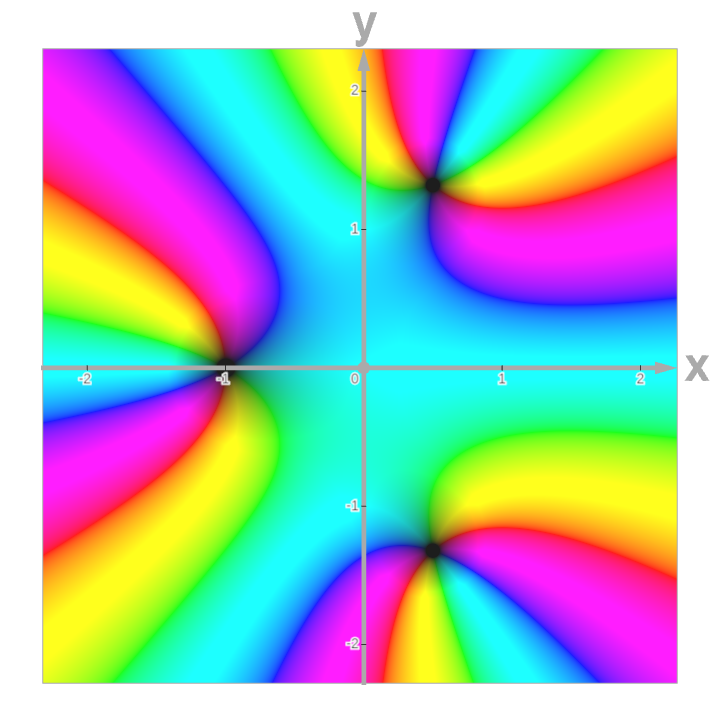
\includegraphics[scale=0.3]{../figures/polynomial_routh_1.png}
\end{center}
\end{minipage}

\par\medskip

da cui notiamo il polo stabile in $p_1 = -1$, e i poli complessi coniugati instabili in $p_{2,3} = \frac{1}{2} \pm \frac{\sqrt{7}}{2}$ (che troviamo anche fattorizzando in $(x + 1) (x^2 - x + 2)$).

\item \textbf{Intera riga nulla:} partiamo dall'esempio del polinomio:
$$
\rho(s) = s^3 + bs^2 + cs + 1
$$
da cui:
$$
\begin{array}{c | c c}
	3 & 1 & c \\
	2 & b & 1 \\
	1 & \frac{bc - 1}{b} \\
	0 & 1
\end{array}
$$
Nel caso $bc = 1$, tutta la riga 1 è nulla.
Questo può essere problematico per la valutazione della stabilità: diciamo allora che con $b, c > 0$, e $bc > 1$, si ha che il polinomio ha solo radici stabili dal primo teorema di Routh.

Per il caso $bc = 1$, invece, possiamo usare più metodi:
\begin{itemize}
	\item Possiamo usare il cosiddetto \textbf{metodo dell'equazione ausiliaria}.
Consideriamo quindi la riga immediatamente superiore a quella nulla:
$$
bs^2 + 1 = 0 \rightarrow s^*_{1, 2} = \pm j \sqrt{ \frac{1}{b} }
$$
avremo che le radici di tale equazione coincidono con le radici mancanti per le quali la tabella non aveva dato soluzioni.
In questo caso, le radici sono complesse coniugate oscillanti, e siamo quindi in condizioni di stabilità.

	\item Il problema del metodo dell'equazione ausiliaria è che ci richiede di risolvere un nuovo polinomio, che nello scorso esempio era semplice (grado 2), ma ptorebbe non esserlo in un caso reale.
Introduciamo quindi il \textbf{metodo della derivata}: prendiamo la derivata rispetto ad $s$ dell'ultima riga e sostituiamo i coefficienti alla riga tutta nulla, cioè scriviamo:
$$
\frac{d}{ds} \left( bs^2 + 1 \right) = 2bs
$$
e quindi sostituiamo:
$$
\begin{array}{c | c c}
	3 & 1 & c \\
	2 & b & 1 \\
	1 & 2b \\
	0 & 1
\end{array}
$$
In questo caso, se la prima colonna modificata non presentà variazioni di segno (è stabile), si ha \textit{stabilità semplice}, mentre se si hanno variazioni di segno abbiamo instabilità per la presenza di poli reali positivi, o poli immaginari con molteplicità $> 1$.

Nell'esempio particolare, abbiamo che con $b<0$ il sistema è instabile, ma ce ne potevamo già accorgere dal fatto che $b<0$ viola le condizioni di applicabilità di Routh.
\end{itemize}

In verità, righe nulle nella matrice di Routh possono derivare solo da casi di \textbf{simmetria quadrantale} delle radici, cioè radici simmetriche rispetto all'asse reale e all'asse immaginario.
Da questa considerazione derivano i criteri precedenti.

Un'ultima considerazione è che, quando si incontrano configurazioni polari con soluzioni immaginarie pure, quello che si trova sono effettivamente le frequenze di oscillazione del sistema, cioè quelle ai limiti della stabilità per cui il sistema dinamico oscilla.
Nel caso precedente avevamo ad esempio trovato che questa era $\omega = \sqrt{\frac{1}{b}}$, dalla coppia di radici complesse coniugate $s^*_{1, 2} = \pm j \sqrt{ \frac{1}{b} }$

\end{itemize}

\subsection{Risposta in frequenza}
Iniziamo quindi a parlare della \textbf{risposta in frequenza} dei sistemi, in particolare con riferimento ai \textit{diagrammi di Bode}.

La risposta in frequenza, detta anche \textit{risposta armonica}, è una proprieta dei sistemi lineari asintoticamente stabili, cioè con poli oscillanti a molteplicità 1 o poli reali non positivi.

\noindent
\begin{minipage}{\textwidth}
I risultati che otterremo si basano sul \textbf{teorema della risposta armonica}:
\begin{theorem}{Teorema della risposta armonica}
Ad un sistema con funzione di trasferimento $G(s)$:
\begin{center}
	\begin{tikzpicture}
		\draw (0,0) rectangle (2, 1);
		\draw[-stealth] (-2, 0.5) -> (0, 0.5);
		\draw[-stealth] (2, 0.5) -> (4, 0.5);
		\node at (1, 0.5) {$G(s)$};
		\node at (-1, 0.7) {$U(s)$};
		\node at (3, 0.7) {$Y(s)$};
	\end{tikzpicture}
\end{center}
se applichiamo un segnale di ingresso sinusoidale:
$$
u(t) = U_M \sin(\omega t)
$$
esaurito il transitorio, l'uscita sarà ancora sinusoidale:
$$
y(t) = |Y(\omega)| \sin\left(\omega t + \phi(\omega)\right)
$$
con pulsazione e fase della sinusoide d'uscita determinati dalla pulsazione della sinusoide di ingresso.
\end{theorem}
\end{minipage}

\par\medskip

Lo scopo dei diagrammi di Bode, vediamo, sarà valutare $Y(\omega)$ e $\phi(\omega)$ al variare della pulsazione $\omega$, o meglio per tutte le pulsazioni $\omega$.

Dimostriamo innanzitutto che una funzione di trasferimento $G(s)$ sottoposta a uno stimolo sinusoidale dà una risposta sinusoidale, cioè prendiamo:
$$
u(t) \sim \sin(\omega t) = \frac{1}{2j} \left( e^{j \omega t} - e^{-j \omega t} \right)
$$
$$
\implies \mathcal{L}\left\{u(t)\right\} = U(s) = \frac{1}{2j} \left( \frac{1}{s- j\omega} - \frac{1}{s + j\omega} \right) = \frac{\omega^2}{s^2 + \omega^2}
$$
L'uscita sarà quindi:
$$
Y(s) = G(s) U(s) = \frac{A_1}{s - j \omega} + \frac{A_1^*}{s + j \omega} + \text{transitori}
$$
vediamo che i transitori vanno a $0$ nel caso di sistemi stabili, in quanto sono in forma $e^{-pt}$ con $p$ positivo, per cui possiamo ignorarli sul lungo termine (come avevamo assunto per ipotesi nella definizione stessa di risposta in frequenza), quindi:
$$
Y(s) \Big|_{t \rightarrow +\infty} = \frac{A_1}{s - j \omega} + \frac{A_1^*}{s + j \omega}
$$
Calcoliamo quindi il residuo $A_1$, consci del fatto che l'altro coefficiente ($A_1^*$) ne sarà semplicemente il coniugato:
$$
A_1 = \lim_{s \rightarrow j \omega} (s - j \omega) G(s) U(s) = (s - j \omega) G(s) \frac{\omega}{(s - j \omega)(s + j \omega)} = G(j \omega) \frac{1}{2j}
$$
e quindi:
$$
A_1^* = -G(-j \omega) \frac{1}{2j}
$$
Troviamo allora la $Y(s)$ a infinito:
$$
Y(s) \Big|_{t \rightarrow +\infty} = \frac{G(j\omega)}{2j} e^{j \omega t} - \frac{G(- j\omega)}{2j} e^{-j \omega t}
$$
Usiamo una semplificazione, visto che la somma di due coniugi dà 2 volte la parte reale di entrambi, cioè:
$$
z + z^* = 2 \mathrm{Re}\left\{z\right\}, \quad \forall z \in \mathbb{C}
$$
e quindi:
$$
G(j \omega) = |G(j \omega)| e^{j \angle G(j \omega)}
$$
che applicando nuovamente la proprietà e sostituendo dà:
$$
Y(s) \Big|_{t \rightarrow +\infty} = 2 \mathrm{Re} \left\{ \frac{G(j \omega)}{2j} e^{j \omega t} \right\} = \mathrm{Re} \left\{ \frac{|G(j \omega)|}{j} e^{j(\omega t + \angle G(j \omega))} \right\}
$$
$$
= \mathrm{Re} \left\{ \frac{|G(\omega)|}{j} \cos(\omega t + \angle G(j \omega)) + |G(j \omega)| \sin(\omega t + \angle G(j \omega)) \right\}
$$
$$
=|G(j \omega)| \sin(\omega t + \angle G(j \omega))
$$
che è esattamente l'ipotesi. \qed

\par\smallskip

Il procedimenti che adotteremo, quindi, è quello di modellare un sistema (che prendiamo come una \textit{scatola nera}) sulla base dalla sua \textit{risposta in frequenza}, magari sfruttando strumenti come l'\textbf{oscilloscopio}:

\begin{center}
	\begin{tikzpicture}
		\draw (0,0) rectangle (2, 1);
		\draw[-stealth] (-2, 0.5) -> (0, 0.5);
		\draw[-stealth] (2, 0.5) -> (4, 0.5);
		\node at (1, 0.5) {$G(s)$};
		\node at (-1, 0.7) {\sffamily{ingresso}};
		\node at (3, 0.7) {\sffamily{uscita}};

		\draw[-stealth] (-1, 0.5) -> (-1, -0.5);
		\draw[-stealth] (3, 0.5) -> (3, -0.5);
		
		\node at (-1, -0.8) {\sffamily{oscilloscopio}};
		\node at (3, -0.8) {\sffamily{oscilloscopio}};
		\node at (-1, -1.15) {\sffamily{di ingresso}};
		\node at (3, -1.15) {\sffamily{di uscita}};
	\end{tikzpicture}
\end{center}

che potrebbero dare misurazioni del tipo:

\begin{center}
	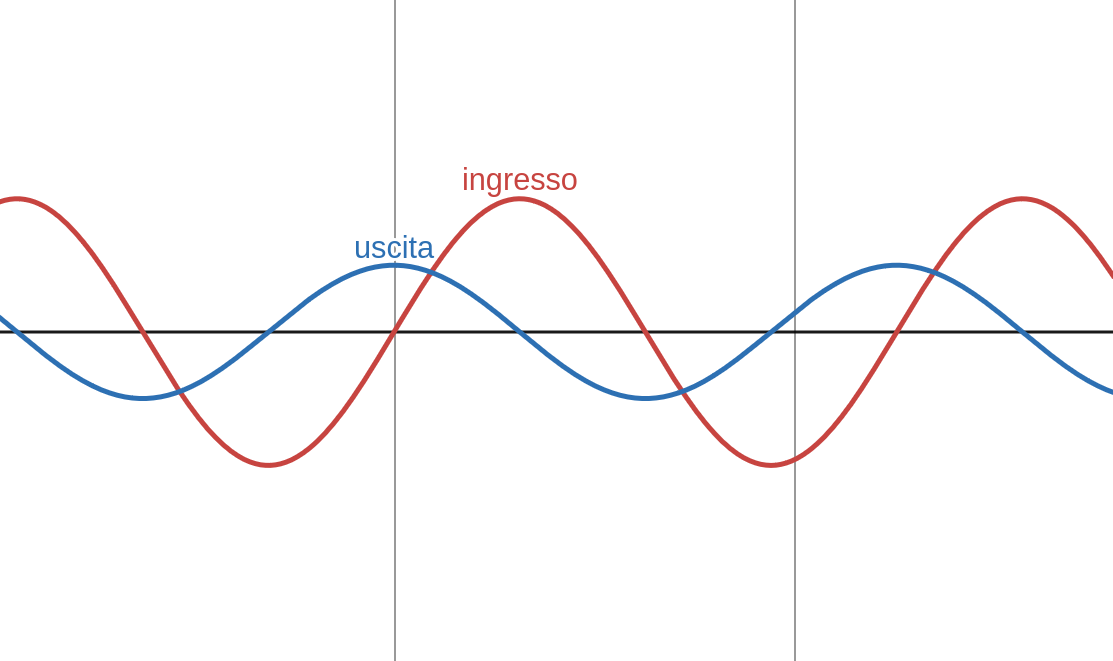
\includegraphics[scale=0.3]{../figures/in_out_sin.png}
\end{center}

Misurazioni di questo tipo evidenziano la variazione di ampiezza e lo scostamento in fase per segnali sinusoidali costanti in frequenza, e facendo più misurazioni per più frequenze si può avere un idea del trasferimento del sistema in dominio frequenze, cioè esattamente la risposta in frequenza.
